\PassOptionsToPackage{unicode=true}{hyperref} % options for packages loaded elsewhere
\PassOptionsToPackage{hyphens}{url}
%
\documentclass[9pt,ignorenonframetext,]{beamer}
\usepackage{pgfpages}
\setbeamertemplate{caption}[numbered]
\setbeamertemplate{caption label separator}{: }
\setbeamercolor{caption name}{fg=normal text.fg}
\beamertemplatenavigationsymbolsempty
% Prevent slide breaks in the middle of a paragraph:
\widowpenalties 1 10000
\raggedbottom
\setbeamertemplate{part page}{
\centering
\begin{beamercolorbox}[sep=16pt,center]{part title}
  \usebeamerfont{part title}\insertpart\par
\end{beamercolorbox}
}
\setbeamertemplate{section page}{
\centering
\begin{beamercolorbox}[sep=12pt,center]{part title}
  \usebeamerfont{section title}\insertsection\par
\end{beamercolorbox}
}
\setbeamertemplate{subsection page}{
\centering
\begin{beamercolorbox}[sep=8pt,center]{part title}
  \usebeamerfont{subsection title}\insertsubsection\par
\end{beamercolorbox}
}
\AtBeginPart{
  \frame{\partpage}
}
\AtBeginSection{
  \ifbibliography
  \else
    \frame{\sectionpage}
  \fi
}
\AtBeginSubsection{
  \frame{\subsectionpage}
}
\usepackage{lmodern}
\usepackage{amssymb,amsmath}
\usepackage{ifxetex,ifluatex}
\usepackage{fixltx2e} % provides \textsubscript
\ifnum 0\ifxetex 1\fi\ifluatex 1\fi=0 % if pdftex
  \usepackage[T1]{fontenc}
  \usepackage[utf8]{inputenc}
  \usepackage{textcomp} % provides euro and other symbols
\else % if luatex or xelatex
  \usepackage{unicode-math}
  \defaultfontfeatures{Ligatures=TeX,Scale=MatchLowercase}
\fi
% use upquote if available, for straight quotes in verbatim environments
\IfFileExists{upquote.sty}{\usepackage{upquote}}{}
% use microtype if available
\IfFileExists{microtype.sty}{%
\usepackage[]{microtype}
\UseMicrotypeSet[protrusion]{basicmath} % disable protrusion for tt fonts
}{}
\IfFileExists{parskip.sty}{%
\usepackage{parskip}
}{% else
\setlength{\parindent}{0pt}
\setlength{\parskip}{6pt plus 2pt minus 1pt}
}
\usepackage{hyperref}
\hypersetup{
            pdftitle={Méthodes de Monte Carlo par chaîne de Markov},
            pdfauthor={Pierre Gloaguen},
            pdfborder={0 0 0},
            breaklinks=true}
\urlstyle{same}  % don't use monospace font for urls
\newif\ifbibliography
\usepackage{longtable,booktabs}
\usepackage{caption}
% These lines are needed to make table captions work with longtable:
\makeatletter
\def\fnum@table{\tablename~\thetable}
\makeatother
\usepackage{graphicx,grffile}
\makeatletter
\def\maxwidth{\ifdim\Gin@nat@width>\linewidth\linewidth\else\Gin@nat@width\fi}
\def\maxheight{\ifdim\Gin@nat@height>\textheight\textheight\else\Gin@nat@height\fi}
\makeatother
% Scale images if necessary, so that they will not overflow the page
% margins by default, and it is still possible to overwrite the defaults
% using explicit options in \includegraphics[width, height, ...]{}
\setkeys{Gin}{width=\maxwidth,height=\maxheight,keepaspectratio}
\setlength{\emergencystretch}{3em}  % prevent overfull lines
\providecommand{\tightlist}{%
  \setlength{\itemsep}{0pt}\setlength{\parskip}{0pt}}
\setcounter{secnumdepth}{0}

% set default figure placement to htbp
\makeatletter
\def\fps@figure{htbp}
\makeatother

\newcommand{\rmd}{\text{d}}
\newcommand{\R}{\mathbb{R}}
\newcommand{\E}{\mathbb{E}}
\newcommand{\V}{\mathbb{V}}
\newcommand{\Unif}{\mathcal{U}}
\newcommand{\Pro}{\mathbb{P}}
\newcommand{\N}{\mathbb{N}}
\newcommand{\Nor}{\mathcal{N}}
\newcommand{\Cov}{\mathbb{C}\text{ov}}
\newcommand{\I}[1]{\mathbf{1}_{#1}}
\newcommand{\e}[1]{\text{e}^{#1}}
\newcommand{\K}{\mathcal{K}}
\newcommand{\seqN}[1]{\left(#1_n\right)_{n\in\N}}
\makeatletter
\let\save@measuring@true\measuring@true
\def\measuring@true{%
  \save@measuring@true
  \def\beamer@sortzero##1{\beamer@ifnextcharospec{\beamer@sortzeroread{##1}}{}}%
  \def\beamer@sortzeroread##1<##2>{}%
  \def\beamer@finalnospec{}%
}
\makeatother

\title{Méthodes de Monte Carlo par chaîne de Markov}
\author{Pierre Gloaguen}
\date{Avril 2020}

\begin{document}
\frame{\titlepage}

\begin{frame}{Rappels des cours précédents}
\protect\hypertarget{rappels-des-cours-pruxe9cuxe9dents}{}

\begin{itemize}
\tightlist
\item
  Méthodes de Monte Carlo pour le calcul d'espérances
\item
  Approche par simulation de vaariables aléatoires i.i.d.
\item
  Méthodes de simulation de loi (échantillons i.i.d.)
\item
  Inférence bayésienne, technique nécessitant des algos de simulations
  de lois
\end{itemize}

\end{frame}

\begin{frame}{Modèle probit}
\protect\hypertarget{moduxe8le-probit}{}

On veut simuler selon une loi
\(\pi(\theta \vert y_{1:n}, \mathbf{x}_{1:n})\) telle que:
\[\pi(\theta \vert y_{1:n}, \mathbf{x}_{1:n}) \propto \text{e}^{-\frac{1}{8}\theta^T\theta}\prod_{k = 1}^n \phi(\mathbf{x}_k^T\theta)^{y_k} (1 - \phi(\mathbf{x}_k^T\theta))^{1 - y_k}\]

\begin{itemize}
\tightlist
\item
  Possible par acceptation rejet si \(n\) n'est pas trop grand;
\item
  Ensuite, ne fonctionne plus \textbf{en pratique} (probabilité
  d'acceptation devient trop faible).
\item
  Nécessité de définir un autre algorithme.
\end{itemize}

\end{frame}

\begin{frame}{Objectif du cours}
\protect\hypertarget{objectif-du-cours}{}

\begin{itemize}
\tightlist
\item
  Présentation des méthodes de Monte Carlo par chaîne de Markov
\item
  Rappel sur les chaînes de Markov (définitions)
\item
  Théorème ergodique
\item
  Algorithme de Metropolis Hastings
\item
  Algorithme de Gibbs
\end{itemize}

\end{frame}

\hypertarget{rappel-sur-les-chauxeenes-de-markov}{%
\section{Rappel sur les chaînes de
Markov}\label{rappel-sur-les-chauxeenes-de-markov}}

\begin{frame}{Chaîne de Markov (à espace d'états fini)}
\protect\hypertarget{chauxeene-de-markov-uxe0-espace-duxe9tats-fini}{}

Soit \(X_0\) une variable aléatoire sur \(\lbrace 1,\dots, K\rbrace\) de
loi \(\pi_0\).

\begin{itemize}
\tightlist
\item
  La suite de variables aléatoires \((X_n)_{n\geq 0}\) à valeurs dans
  \(\K =\lbrace 1,\dots, K\rbrace\) est une chaîne de Markov si pour
  tout \(n\geq 1\) est pour tout suite \((k_0,\dots,k_n)\) d'éléments de
  \(\K\), on a :
\end{itemize}

\[\mathbb{P}\left( X_n = k_n \vert X_0 = k_0,\dots,X_{n- 1} = k_{n- 1}\right) = \mathbb{P}(X_n = k_n \vert X_{n-1} = k_{n-1})\]

\begin{itemize}
\tightlist
\item
  Cette chaîne est \(\textit{homogène}\) si, pour (\(i, j\)) dans
  \(\K \times \K\):
  \(\mathbb{P}(X_n = j \vert X_{n-1} = i) = \mathbb{P}(X_1 = j \vert X_{0} = i) = P_{ij}\)
\item
  La matrice \(P = (P_{ij})\) est la \textbf{matrice de transition} de
  la chaîne de Markov.
\item
  Une chaîne de Markov homogène est entièrement caractérisée par
  \(\pi_0\) et \(P\).
\end{itemize}

\end{frame}

\begin{frame}{Loi de la chaîne}
\protect\hypertarget{loi-de-la-chauxeene}{}

Pour \(n \geq 0\), on note \(\pi_n\), la loi de l'état \(X_n\), c'est à
dire le vecteur ligne
\[\pi_n = (\pi_{n,1} = \Pro(X_n = 1),\dots,\pi_{n, K} = \Pro(X_n = K)).\]
On a:

\begin{itemize}
\tightlist
\item
  \(\Pro(X_1 = j) = \sum_{i = 1}^k \Pro(X_0 = i) \times \Pro(X_1 = j \vert X_0 = i) = \sum_{i = 1}^k \pi_{0,i}P_{ij}\)
  Cette relation est résumée par l'équation \(\pi_1 = \pi_0P\)
\item
  Par récurrence, on montre que
  \[P^{(n)}_{ij} := \Pro(X_n = j\vert X_0 = i) = (P^n)_{ij}\] où \(P^n\)
  est la puissance \(n\)-ième de la matrice \(P\).
\item
  Ainsi: \[\pi_n = \pi_0P^n\]
\end{itemize}

\end{frame}

\begin{frame}{Mesure invariante pour \(P\)}
\protect\hypertarget{mesure-invariante-pour-p}{}

Soit \(\pi\) un vecteur (ligne) de probabilité sur \(\K\).

\begin{itemize}
\item
  \(\pi\) est une \textbf{mesure invariante pour la chaîne de Markov de
  transition \(P\)} si: \[\pi P = \pi\] \pause
\item
  Si \(\pi_0\) est une mesure invariante pour \(P\), alors, pour tout
  \(n\), \(\pi_n = \pi_0\).
\item
  Dans ce cas, les V.A. \(X_0,\dots, X_n\) sont identiquement
  distribuées (mais pas indépendantes!).
\end{itemize}

\end{frame}

\begin{frame}{Irréductibilité}
\protect\hypertarget{irruxe9ductibilituxe9}{}

Une chaîne de Markov homogène sur \(\K\), de transition \(P\) est
\textbf{irréductible} si
\[\forall i,j \in \K\times \K,~\exists~n \text{ tel que } P^{(n)}_{i,j} > 0\]

\begin{itemize}
\tightlist
\item
  Pour deux états de la chaîne, il est possible d'accéder de l'un à
  l'autre en un temps fini.
\end{itemize}

\end{frame}

\begin{frame}{Apériodicité}
\protect\hypertarget{apuxe9riodicituxe9}{}

Soit \((X_n)_{n\geq 1}\) une chaîne de Markov homogène sur \(\K\). Pour
\(k \in \K\),

\begin{itemize}
\tightlist
\item
  La \emph{période} de l'état \(k\), notée \(d(k)\), est le P.G.C.D. de
  tous les entiers \(n\) tels que \(P^{(n)}_{kk} > 0\) (avec la
  convention \(pgcd(\emptyset) = +\infty\)):
  \[d(j) = pgcd\left\lbrace n\geq 1, P^{(n)}_{kk} > 0\right\rbrace\] Une
  chaîne est dite apériodique si pour tout \(k\) dans \(\K\),
  \(d(k) = 1\). \pause 
\end{itemize}

Pour une chaîne irréductible, une condition suffisante pour être
apériodique est qu'il existe un \(k\in \K\) tel que \(P_{kk} > 0\).

\end{frame}

\hypertarget{thuxe9oruxe8me-ergodique}{%
\section{Théorème ergodique}\label{thuxe9oruxe8me-ergodique}}

\begin{frame}{Théorème ergodique}
\protect\hypertarget{thuxe9oruxe8me-ergodique-1}{}

Soit \((X_n)_{n\geq 0}\) une chaîne de Markov sur \(\K\) de loi initiale
\(\pi_0\) et de matrice de transition \(P\). On suppose que cette chaîne
est irréductible et apériodique. Alors: \pause

\begin{enumerate}
\tightlist
\item
  Cette chaîne de Markov admet une unique mesure de probabilité
  invariante \(\pi\). \pause
\item
  \(X_n \overset{loi}{\longrightarrow} X\) où \(X\) est une v.a. de loi
  \(\pi\).\pause
\item
  Pour toute fonction \(\varphi\) intégrable par rapport à \(\pi\), on a
  :
  \[\frac{1}{M + 1} \sum_{k = 0}^M \varphi(X_k) \underset{M \rightarrow +\infty}{\overset{p.s.}{\longrightarrow}} \mathbb{E}_\pi[\varphi(X)].\]
  \pause
\item
  Si \(\varphi(X)\) admet un moment d'ordre supérieur à 2, on a
  \[\sqrt{M}\left( \frac{1}{M + 1}\sum_{k = 0}^n \varphi(X_k) - \mathbb{E}_\pi[\varphi(X)] \right) \underset{M \rightarrow +\infty}{\overset{Loi}{\longrightarrow}} \mathcal{N}(0, \sigma^2)\]
\end{enumerate}

\pause

Une propriété analogue reste vraie quand la chaîne de Markov est à
valeurs dans un ensemble continu (typiquement, \(\R^d\)).

\end{frame}

\begin{frame}{Conséquence et intérêt pratique du théorème ergodique}
\protect\hypertarget{consuxe9quence-et-intuxe9ruxeat-pratique-du-thuxe9oruxe8me-ergodique}{}

\begin{itemize}
\tightlist
\item
  Pour estimer \(\mathbb{E}_\pi[\varphi(X)]\), il suffit d'être capable
  de simuler une chaîne de Markov apériodique et irréductible de mesure
  de probabilité invariante \(\pi\).\pause 
\item
  Il n'est pas nécessaire de savoir tirer selon \(\pi\) directement!
  \pause
\item
  Le point 2. dit qu'\emph{au bout d'un certain temps}, les \(X_n\)
  simulés pourront être considérés comme de loi \(\pi\) (mais pas
  indépendants!)! \pause
\item
  Encore faut il être capable de construire une chaîne de Markov
  apériodique, irréductible, de loi invariante donnée par \(\pi\)!\pause
\item
  \(\longrightarrow\) Algorithme de Metropolis Hastings
\end{itemize}

\end{frame}

\begin{frame}{Remarque sur le Théorème Central Limite}
\protect\hypertarget{remarque-sur-le-thuxe9oruxe8me-central-limite}{}

\begin{itemize}
\tightlist
\item
  Les V.A. dans l'estimateur Monte Carlo ne sont plus indépendantes.
\item
  \(\Rightarrow\) la variance \(\sigma^2\) n'est absolument pas triviale
  (il ne s'agit pas de \(\V[\varphi(X)]\))!
\item
  Pas nécessairement facile à estimer!
\item
  Ainsi, avoir un IC asymptotique sur \(\mathbb{E}_\pi[\varphi(X)]\)
  n'est plus du tout immediat.
\end{itemize}

\end{frame}

\hypertarget{algorithme-de-metropolis-hastings}{%
\section{Algorithme de Metropolis
Hastings}\label{algorithme-de-metropolis-hastings}}

\begin{frame}{Réversibilité}
\protect\hypertarget{ruxe9versibilituxe9}{}

Soit \(\pi =(\pi_1,\dots, \pi_K)\) une mesure de probabilité sur \(\K\)
et \((X_n)_{n\geq 0}\) une chaîne de Markov homogène de matrice de
transition \(P\) et de loi initiale \(\pi_0\).\pause 

\begin{itemize}
\item
  \(\pi\) est \textbf{réversible} pour \(P\) si elle vérifie la
  condition d'équilibre:
  \[\forall (i, j) \in \K\times \K,~\pi_i \times P_{ij} = \pi_j \times P_{ji}\]
\item
  \emph{Propriété:} Si \(\pi\) est réversible pour une chaîne de Markov
  de transition \(P\), alors, \(\pi\) est une mesure de probabilité
  invariante pour \(P\).\pause
\item
  \emph{Preuve} Soit \(\pi\) une mesure de probabilité réversible pour
  \(P\). On a tout de suite que \begin{align*}
  \forall j \in \K~~(\pi P)_j & = \sum_{i = 1}^{K} \pi_i P_{ij}& \\
  &= \sum_{i = 1}^{K} \pi_j P_{ji} &\text{ par réversibilité}\\
  &= \pi_j &\text{ par propriété de } P\\
  \Rightarrow \pi P &= \pi&
  \end{align*}
\end{itemize}

\end{frame}

\begin{frame}{Objectif de l'algorithme}
\protect\hypertarget{objectif-de-lalgorithme}{}

\begin{itemize}
\tightlist
\item
  On veut simuler selon la loi \(\pi\).
\item
  Construire une chaîne de Markov irréductible et apériodique, de loi
  initiale \(\pi_0\) et de transition \(P\), \textbf{réversible pour P}
\item
  On va se servir pour ça d'une chaîne de Markov de transition \(Q\)
  (réversible et apériodique) \textbf{parcourant le même espace que
  \(P\)} (le support de \(\pi\)).
\end{itemize}

\end{frame}

\begin{frame}{Algorithme de Metropolis Hastings (formulation discrete)}
\protect\hypertarget{algorithme-de-metropolis-hastings-formulation-discrete}{}

\begin{itemize}
\tightlist
\item
  Soit \(Q\) une matrice stochastique \(K \times K\) satisfaisant la
  condition suivante:
  \[\forall (i, j) \in \K\times \K, Q_{ij} > 0 \Leftrightarrow Q_{ji} > 0\]
\item
  Soit \((X_n)_{n\geq 0}\) la suite de variables aléatoires construite
  ainsi:\pause
\end{itemize}

\begin{enumerate}
\tightlist
\item
  On simule \(X_0\) selon \(\pi_0\).\pause
\item
  Pour \(n\geq 1\):
\end{enumerate}

\begin{enumerate}
[a.]
\tightlist
\item
  On tire \(Y_n\) selon la loi \(Q_{X_{n-1}\bullet}\) (la ligne de \(Q\)
  donnée par \(X_{n-1}\)).\pause
\item
  On tire une loi uniforme \(U\) indépendante de \(Y_n\).\pause
\item
  On calcule la quantité
  \[\alpha(X_{n-1}, Y_n) = \min\left(1, \frac{\pi_{Y_n}Q_{Y_n X_{n-1}}}{\pi_{X_{n - 1}}Q_{X_{n-1}Y_n}}\right)\]
  \pause
\item
  On pose: \[X_n = \left\lbrace
  \begin{array}{lr}
  Y_n & \text{ si } U\leq\alpha(X_{n-1}, Y_n)\\
  X_{n - 1} &\text{ sinon}
  \end{array}
   \right.\]\pause
\end{enumerate}

\begin{itemize}
\tightlist
\item
  \textbf{Propriété 1:} \((X_n)_{n \geq 1}\) est une chaîne de Markov de
  transition \(P\) où
  \[P_{ij} = Q_{ij}\alpha(i, j)  \text{ si } i\neq j,~~ P_{jj} = 1 - \sum_{j\neq i} P_{ij}\]
\item
  \textbf{Propriété 2:} De plus \textbf{\(\pi\) est invariante pour
  \(P\).}
\end{itemize}

\end{frame}

\begin{frame}{Preuve}
\protect\hypertarget{preuve}{}

\begin{block}{Matrice de transition \(P\)}

On veut montrer que:
\[P_{ij} = Q_{ij}\alpha(i, j)  \text{ si } i\neq j,~~ P_{jj} = 1 - \sum_{j\neq i} P_{ij}\]
\pause Soit \(i\neq j\): \begin{align*}
\Pro(X_{n} = j \vert X_{n -1} = i) &= \Pro\left(Y_{n} = j , U\leq \alpha(X_{n-1}, Y_{n})\vert X_{n -1} = i \right)\\
&=  \Pro\left(Y_{n} = j , U\leq \alpha(i, j)\vert X_{n -1} = i \right)\\
&=\Pro\left( U\leq \alpha(i, j)\vert X_{n -1} = i, Y_n = j \right)\Pro\left(Y_{n} = j \vert X_{n-1} = i\right)\\
&= Q_{ij}\alpha(i,j)
\end{align*}

\end{block}

\end{frame}

\begin{frame}{Preuve que \(\pi\) est mesure invariante}
\protect\hypertarget{preuve-que-pi-est-mesure-invariante}{}

Il suffit de montrer que \(\pi\) est réversible pour \(P\).

Soient \(i\neq j \in \K\):\pause 

\begin{align*}
\pi_iP_{ij} &=  \pi_i Q_{ij}\alpha(i, j)\\
&= \pi_i Q_{ij} \min\left(1, \frac{\pi_{j}Q_{ji}}{\pi_{i}Q_{ij}}\right)\\
&= \min\left(\pi_i Q_{ij}, \pi_{j}Q_{ji}\right)\\
&= \pi_{j}Q_{ji}\min\left(\frac{\pi_i Q_{ij}}{ \pi_{j}Q_{ji}}, 1 \right)\\
&= \pi_{j}Q_{ji}\alpha(j,i)\\
&=\pi_{j}P_{ji}
\end{align*}

\end{frame}

\begin{frame}{Algorithme dans le cas continu}
\protect\hypertarget{algorithme-dans-le-cas-continu}{}

Supposons qu'on veuille simuler dans \(\R^d\) selon une densité \(\pi\),
éventuellement connue à une constante près, c'est à dire que
\[\forall x \in \R^d,~\pi(x) = \frac{\tilde{\pi}(x)}{\int_{\R^d}\tilde{\pi}(z)\rmd z}\]
On remplace alors la matrice de transition par un
\(\textit{noyau de transition}\) sur \(\R^d\), à savoir une fonction
\begin{equation*}
\begin{array}{lccc}
q:& \R^d\times \R^d &\mapsto& \R_+\\
& (x, y) & \mapsto & q(x, y)\geq 0
\end{array}
\end{equation*} telle que \(\int_{\R^d}q(x, y)\rmd y = 1\) (typiquement,
la loi d'une marche aléatoire centrée en \(x\).\pause

Si on sait simuler, pour \(x\) fixé, selon \(q\), et qu'on a
\(q(x, y) > 0 \Leftrightarrow q(y, x) > 0\), alors, l'algorithme de
Metropolis reste valide en remplaçant \(\pi\) par \(\tilde{\pi}\) et
\(Q\) par \(q\). \pause

\begin{itemize}
\tightlist
\item
  Le ratio ne nécessite pas la constante de normalisation car
  \[\frac{\tilde{\pi}(y)}{\tilde{\pi}(x)} = \frac{\pi(y)}{\pi(x)}\]
\end{itemize}

\end{frame}

\hypertarget{exemple-2-cas-non-conjuguuxe9}{%
\section{Exemple 2: cas non
conjugué}\label{exemple-2-cas-non-conjuguuxe9}}

\begin{frame}{Exemple: Prédiction de présence d'oiseaux}
\protect\hypertarget{exemple-pruxe9diction-de-pruxe9sence-doiseaux}{}

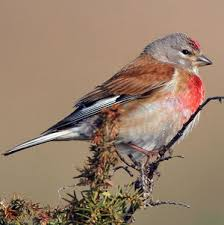
\includegraphics[width = 0.3\textwidth]{figures/linotte.jpeg}

Une étude consiste en l'observation de la présence ou non de la linotte
mélodieuse sur différents sites échantillonnés.

\begin{block}{Caractéristiques des sites}

Sur ces 300 sites sont mesurées différentes caractéristiques:

\begin{itemize}
\tightlist
\item
  Le nombre de vers moyens sur une surface au sol de \(1m^2\).
  (Covariable 1)
\item
  La hauteur d'herbe moyenne sur une surface au sol de \(1m^2\).
  (Covariable 2)
\item
  On calcule cette hauteur d'herbe au carré. (Covariable 3).
\end{itemize}

\end{block}

\end{frame}

\begin{frame}{Données}
\protect\hypertarget{donnuxe9es}{}

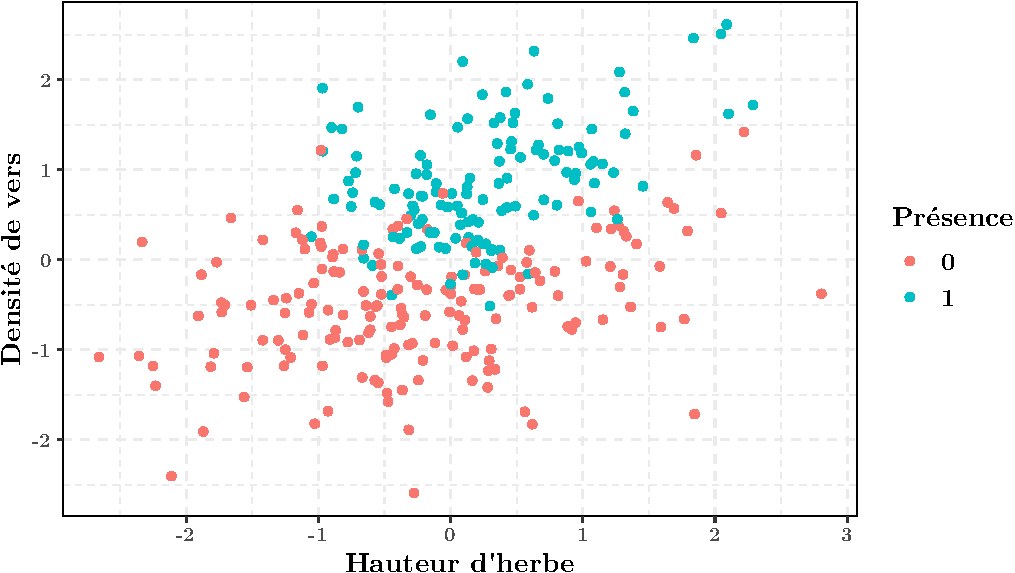
\includegraphics{diapos_mcmc_files/figure-beamer/plot_donnees_presence-1.pdf}

\end{frame}

\begin{frame}{Notations et modèle de régression probit}
\protect\hypertarget{notations-et-moduxe8le-de-ruxe9gression-probit}{}

On note \(y_1, \dots, y_n\) les observations de présence (1 si on
observe un oiseau, 0 sinon) sur les sites \(1\) à \(n\).

On note
\[\mathbf{x}_k = (\overset{\text{Nb. vers}}{x_{k,1}}, \overset{\text{Haut. herbe}}{x_{k,2}}, \overset{\text{Haut. herbe}^2}{x_{k,3}})^T\]
le vecteur des covariables sur le \(k\)-ème site
\((1\leq k \leq n)\).\pause

On pose le modèle suivant:

\(Y_k \sim \mathcal{B}ern(p_k)\) où
\[p_k = \phi(\beta_0 + \beta_1 x_{i1} + \beta_2x_{i2} + \beta_3 x_{i3}) = \phi(\mathbf{x}_k^T\theta),\]
où

\begin{itemize}
\tightlist
\item
  \(\phi\) est la fonction de répartition d'une \(\mathcal{N}(0, 1)\),
  i.e.
  \[\phi(z) = \frac{1}{\sqrt{2\pi}}\int_{-\infty}^z \text{e}^{-\frac{u^2}{2}}\text{d}u\]
\item
  \(\theta = \left\lbrace \beta_0, \beta_1, \beta_2, \beta_3\right\rbrace\)
  est le vecteur des paramètres à estimer.
\end{itemize}

\end{frame}

\begin{frame}{Modèle Bayésien}
\protect\hypertarget{moduxe8le-bayuxe9sien}{}

\begin{block}{Prior sur \(\theta\)}

Comme a priori sur \(\theta\), on choisit une normale avec une grande
variance\(\theta \overset{\text{prior}}{\sim} \mathcal{N}(0, 4 I),\)
donc
\[\pi(\theta) = \frac{1}{\sqrt{2\pi \times 4}^4} \text{e}^{-\frac{1}{8}\theta^T\theta}\]
où \(I\) est la matrice Identité (ici \(4 \times 4\)) \pause

\end{block}

\begin{block}{Vraisemblance}

Pour un vecteur d'observations \(y_{1:k}\), la vraisemblance
\[L(y_{1:k}\vert \theta) = \prod_{k = 1}^n \underset{\text{Proba. présence}}{\phi(\mathbf{x}_k^T\theta)^{y_k}}\times \underset{\text{Proba. absence}}{(1 - \phi(\mathbf{x}_k^T\theta))}^{1 - y_k}\]
\pause

\end{block}

\begin{block}{Posterior}

Le posterior est donc donné par:
\[\pi(\theta \vert y_{1:n}) \propto \pi(\theta) L(y_{1:n}\vert \theta) \propto \text{e}^{-\frac{1}{8}\theta^T\theta} \prod_{k = 1}^n \phi(\mathbf{x}_k^T\theta)^{y_k} (1 - \phi(\mathbf{x}_k^T\theta))^{1 - y_k}\]

\end{block}

\end{frame}

\begin{frame}{Algorithme de Metropolis Hastings}
\protect\hypertarget{algorithme-de-metropolis-hastings-1}{}

La loi stationnaire cible est \(\pi(\mathbf{y}\vert \theta)\). Pour
\(n = 300\), l'acceptation rejet vu au cours précédent fonctionnera très
mal en pratique. \pause

On fait un algorithme de Metropolis Hastings avec comme loi de
proposition une marche aléatoire dans \(\mathbb{R}^4\), de matrice de
covariance \(\tau^2\times I_4\).

\end{frame}

\begin{frame}{Résultat d'un algorithme lancé depuis un point de départ}
\protect\hypertarget{ruxe9sultat-dun-algorithme-lancuxe9-depuis-un-point-de-duxe9part}{}

\begin{itemize}
\tightlist
\item
  On choisit \(\beta^{(0)} = (0, 0, 0, 0)\) et \(\tau^2 = 0.1\), on
  lance 1000 itérations.
\end{itemize}

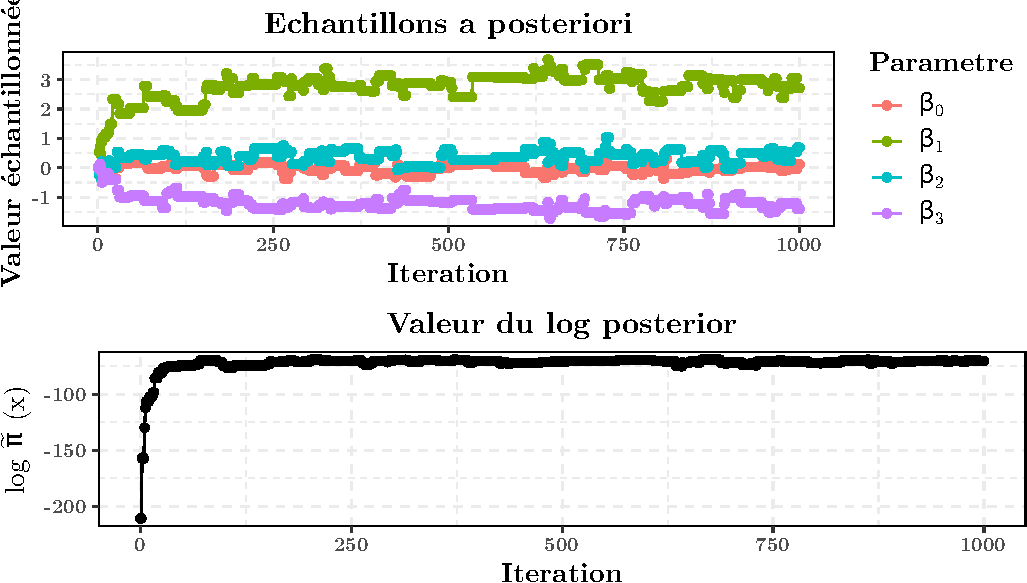
\includegraphics{diapos_mcmc_files/figure-beamer/plot_premier_mcmc-1.pdf}

\end{frame}

\begin{frame}{Sensibilité au point de départ}
\protect\hypertarget{sensibilituxe9-au-point-de-duxe9part}{}

Il faut toujours vérifié la sensibilité au point de départ!

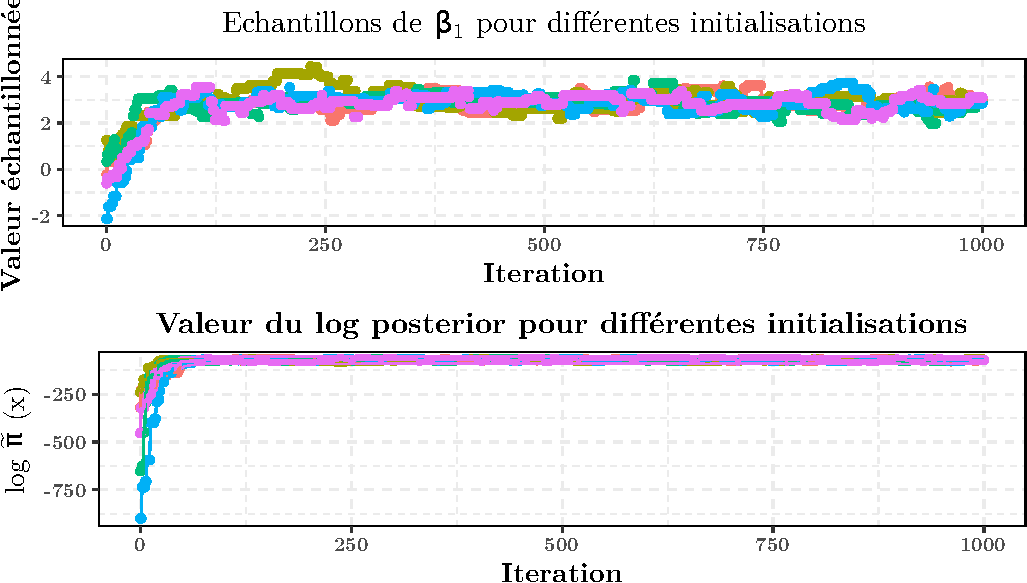
\includegraphics{diapos_mcmc_files/figure-beamer/plot_mcmc_multiple_start-1.pdf}

\end{frame}

\begin{frame}{Influence de \(\tau^2\)}
\protect\hypertarget{influence-de-tau2}{}

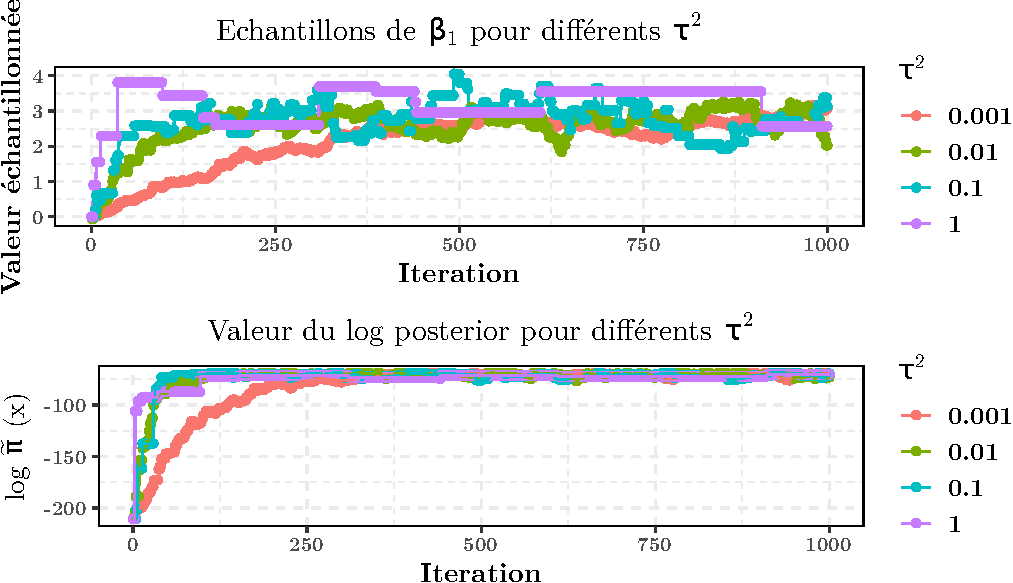
\includegraphics{diapos_mcmc_files/figure-beamer/plot_mcmc_multiple_tau-1.pdf}

\end{frame}

\begin{frame}{Influence de \(\tau^2\)}
\protect\hypertarget{influence-de-tau2-1}{}

\textbf{Taux d'acceptation dans l'algorithme}

\begin{longtable}[]{@{}rr@{}}
\toprule
\(\tau^2\) & Taux d'acceptation\tabularnewline
\midrule
\endhead
0.001 & 0.781\tabularnewline
0.010 & 0.515\tabularnewline
0.100 & 0.147\tabularnewline
1.000 & 0.013\tabularnewline
\bottomrule
\end{longtable}

\pause

\textbf{Autocorrelation dans les chaînes}

Correlation entre empirique entre \(\beta_1^{n}\) et
\(\beta_1^{(n + 1)}\)

\begin{longtable}[]{@{}rr@{}}
\toprule
\(\tau^2\) & Autocorrelation\tabularnewline
\midrule
\endhead
0.001 & 0.9993751\tabularnewline
0.010 & 0.9917581\tabularnewline
0.100 & 0.9835038\tabularnewline
1.000 & 0.9864433\tabularnewline
\bottomrule
\end{longtable}

\end{frame}

\begin{frame}{Reduction de l'autocorrelation}
\protect\hypertarget{reduction-de-lautocorrelation}{}

En pratique, on choisira une fracion des points. On appelle cela le
\textbf{thinning}.\pause

Autocorrélation en prenant un point sur 100.

\begin{longtable}[]{@{}rr@{}}
\toprule
\(\tau^2\) & Autocorrelation\tabularnewline
\midrule
\endhead
0.001 & 0.8092081\tabularnewline
0.010 & 0.2395796\tabularnewline
0.100 & 0.1502224\tabularnewline
1.000 & 0.3861150\tabularnewline
\bottomrule
\end{longtable}

\end{frame}

\begin{frame}{Estimation de la loi}
\protect\hypertarget{estimation-de-la-loi}{}

Les premières valeurs n'ont aucune raison d'être tirées selon la loi
cible.

En pratique, on les supprimera. On appelle cela le
\textbf{burn-in}.\pause

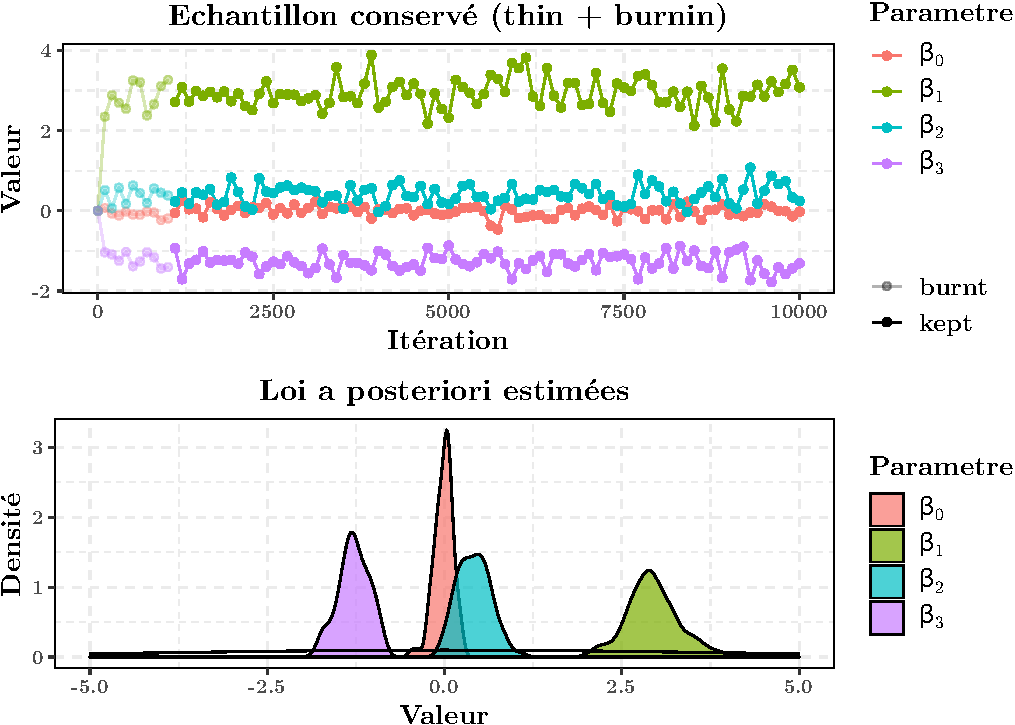
\includegraphics{diapos_mcmc_files/figure-beamer/plot_burned_thin-1.pdf}

\end{frame}

\hypertarget{autres-algorithmes-mcmc}{%
\section{Autres algorithmes MCMC}\label{autres-algorithmes-mcmc}}

\begin{frame}{Echantillonneur de Gibbs}
\protect\hypertarget{echantillonneur-de-gibbs}{}

\begin{itemize}
\item
  Utile quand \(\theta\) est en grande dimension;
\item
  On suppose qu'on sait simuler selon les loi conditionnelles de
  \(\theta\)\pause
\item
  Soit \(X\) un vecteur aléatoire en dimension \(d\)
  \(X = (X^{(1)},\dots, X^{(d)})\).
\item
  On note
  \(X^{-(\ell)} = (X^{(1)},\dots, X^{(\ell-1)}, X^{(\ell+1)}, X^{(d)})\),
\item
  Si on sait simuler la variable aléatoire
  \(X^{(\ell)}\vert X^{(-\ell)}\), l'algo est le suivant:

  \begin{enumerate}
  \item Prendre $X_0 = (X_0^{(1)},\dots, X_0^{(d)})$ tiré selon une loi initiale.
  \item Pour $k \geq 1$:
  \begin{enumerate}
  \item Tirer $\ell$ uniformément dans $\lbrace1,\dots,d\rbrace$;
  \item Simuler $Y$ selon la loi $X^{(\ell)} \vert \lbrace X^{(-\ell)} = X_{k-1}^{(-\ell)} \rbrace$
  \item Poser $X_k = (X_{k - 1}^{(1)},\dots, X_{k-1}^{(\ell-1)}, Y, X_{k - 1}^{(\ell+1)}, X_{k-1}^{(d)})$
  \end{enumerate}
  \end{enumerate}
\end{itemize}

\end{frame}

\begin{frame}{Propriété de l'échantillonneur de Gibbs}
\protect\hypertarget{propriuxe9tuxe9-de-luxe9chantillonneur-de-gibbs}{}

\begin{itemize}
\tightlist
\item
  L'échantillonneur de Gibbs est équivalent à un algorithme de
  Metropolis Hastings où la quantité \(\alpha\) est toujours égale à 1,
\item
  C'est à dire un Metropolis Hastings où on n'accepte tous les
  candidats!
\item
  Algorithme utile dès que la simulation des lois conditionnelles est
  faisable.
\item
  Si les lois conditionnelles induisent une matrice de transition (ou un
  noyau) de Markov irréductible et apériodique, alors le théorème
  ergodique s'applique.
\end{itemize}

\end{frame}

\end{document}
